\providecommand{\main}{..} 
\documentclass[\main/boa.tex]{subfiles}

\begin{document}

\section{Analiza danych obserwacyjnych zwiedzających wystawy w Centrum Nauki Kopernika}


\begin{minipage}{0.915\textwidth}
	\centering
  {\bf \LARGE \index[a]{Wróblewska Anna} Anna Wróblewska}
\end{minipage}


\begin{affiliations}
\begin{minipage}{0.915\textwidth}
\centering
\large MiNI, Politechnika Warszawska  \\[1pt]
Kontakt: \href{mailto:awroble@gmail.com}{\nolinkurl{awroble@gmail.com}}\\
\end{minipage}
\end{affiliations}

W prezentacji podsumowujemy współpracę z Centrum Nauki Kopernik (CNK) \break (Katarzyna Potęga), Uniwersytetem Nauk Społecznych i Humanistycznych (Łukasz Tanaś) oraz Wydziałem Matematyki i Nauk Informacyjnych Politechniki Warszawskiej (WUT). Pracowaliśmy nad danymi obserwacyjnymi zebranymi podczas testów przeprowadzonych w CNK. Dane te zostały przeanalizowane przez studentów nowej specjalności \break Przetwarzanie i analiza danych na wydziale MINI PW.
Dane zostały zebrane z trzech badań obserwacyjnych dotyczących zachowania dzieci i rodziców oraz dzieci szkolnych, a także testów dotyczących rozpoznawania i zrozumienia emocji.
Postawiliśmy wiele hipotez i pytań badawczych, zweryfikowaliśmy je w oparciu o dostępne dane, np. podsumujemy różne postawy rodziców, a także zaufanie i rozpoznanie emocji oraz zaangażowanie dzieci w oglądane/doświadczane eksponaty. 

\bio
\begin{wrapfigure}{r}{100px}
    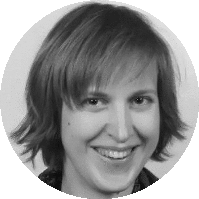
\includegraphics[width=100px]{img/guests/czarno_biale/awroblewska.png}
\end{wrapfigure} 
Anna Wróblewska otrzymała doktorat w dziedzinie informatyki w 2008 roku na Wydziale Elektroniki i Technik Informacyjnych Politechniki. Pracuje jako adiunkt na Politechnice Warszawskiej, wcześniej w Instytucie Informatyki Politechniki Warszawskiej, obecnie na Wydziale Matematyki i Nauk Informacyjnych, w tym prowadzi zajęcia na kierunku Informatyka na nowej specjalności Przetwarzanie i Analiza Danych (Data Science). Prowadzi projekty studenckie, prace magisterskie i inżynierskie, wykłady z zakresu eksploracji danych tekstowych i uczenia maszynowego.

Posiada kilkuletnie doświadczenie w projektowaniu inteligentnych systemów analizy i opisu semantycznego danych nabyte w środowisku komercyjnym i naukowym. Obecnie od ponad 3 lat pracuje na stanowisku ekspert analizy danych (Data Scientist) w firmie Allegro – największym portalu e-commerce w Europie Wschodniej, gdzie zajmuje się metodami analizy danych także tekstowych i obrazowych.

Ponadto jest autorką ponad 35 publikacji w polskich i międzynarodowych czasopismach i materiałach. Jej zainteresowania naukowe koncentrują się wokół uczenia maszynowego w praktycznych zastosowaniach, w tym przede wszystkim semantycznego rozumienia danych: tekstu i obrazu, budowania ontologii, wyszukiwania semantycznego, systemów rekomendacyjnych. Prywatnie jest szczęśliwą żoną i mamą dzieci w wieku od przedszkolaka do nastolatka.

\end{document}
